\documentclass[11pt]{article}

\usepackage[utf8]{inputenc}
\usepackage[T1]{fontenc}
\usepackage[spanish]{babel}
\usepackage[margin=2.5cm]{geometry}
\usepackage{hyperref}
\usepackage{url}
\usepackage{booktabs}
\usepackage{amsfonts}
\usepackage{amsmath}
\usepackage{amssymb}
\usepackage{nicefrac}
\usepackage{microtype}
\usepackage{graphicx}
\usepackage{subcaption}
\usepackage{float}
\usepackage{titling}
\usepackage{abstract}
\usepackage{xcolor}
\usepackage{listings}

\renewcommand{\abstractnamefont}{\normalfont\bfseries}
\renewcommand{\abstracttextfont}{\normalfont\small\itshape}

% --- Estilo para el codigo Python ---
\definecolor{codegreen}{rgb}{0.0,0.5,0.0}
\definecolor{codegray}{rgb}{0.5,0.5,0.5}
\definecolor{codepurple}{rgb}{0.58,0.0,0.82}
\definecolor{backcolour}{rgb}{0.96,0.96,0.94}

\lstdefinestyle{python}{
  backgroundcolor=\color{backcolour},
  commentstyle=\color{codegreen}\itshape,
  keywordstyle=\color{blue},
  stringstyle=\color{codepurple},
  basicstyle=\ttfamily\footnotesize,
  breakatwhitespace=false,
  breaklines=true,
  captionpos=b,
  keepspaces=true,
  numbers=left,
  numbersep=6pt,
  numberstyle=\tiny\color{codegray},
  showspaces=false,
  showstringspaces=false,
  showtabs=false,
  tabsize=4,
  frame=single,
  language=Python,
}
\lstset{style=python}

\graphicspath{{output/}}

\title{\textbf{TP 2.2 - Generadores de n\'umeros pseudoaleatorios de
distintas distribuciones de probabilidad}}

\author{
  Agustin Santinelli \\
  Ingenier\'ia en Sistemas de Informaci\'on \\
  Universidad Tecnol\'ogica Nacional \\
  Legajo 52211 \\
  \texttt{agustinsantinelli@gmail.com}
  \and
  Joaquin Peralta \\
  Ingenier\'ia en Sistemas de Informaci\'on \\
  Universidad Tecnol\'ogica Nacional \\
  Legajo 52151 \\
  \texttt{joaaperalta@gmail.com}
  \and
  Martin Ratti \\
  Ingenier\'ia en Sistemas de Informaci\'on \\
  Universidad Tecnol\'ogica Nacional \\
  Legajo 52398 \\
  \texttt{martinratti10@gmail.com}
  \and
  Tomas Levrand \\
  Ingenier\'ia en Sistemas de Informaci\'on \\
  Universidad Tecnol\'ogica Nacional \\
  Legajo 52206 \\
  \texttt{tomylevrand@gmail.com}
}

\date{\today}

\begin{document}
\maketitle

\begin{abstract}
\noindent A partir del Generador Congruencial Lineal validado en el TP 2.1
se construyen generadores de nueve distribuciones de probabilidad --- cuatro
continuas (uniforme, exponencial, gamma y normal) y cinco discretas
(Pascal, binomial, hipergeom\'etrica, Poisson y emp\'irica discreta) ---
siguiendo los m\'etodos del cap\'itulo 4 de Naylor. Para cada distribuci\'on
se presenta su fundamento te\'orico, la derivaci\'on de la funci\'on de
distribuci\'on acumulada y su inversa cuando corresponde, el c\'odigo
Python de generaci\'on y, para las distribuciones que el enunciado exige
testear, una prueba de bondad de ajuste (Kolmogorov-Smirnov para las
continuas, chi-cuadrado para las discretas). Los resultados confirman que
todas las distribuciones generadas reproducen fielmente su comportamiento
te\'orico: las medias y varianzas emp\'iricas coinciden con las esperadas
y las seis pruebas exigidas se superan al nivel $\alpha = 0{,}05$.

\vspace{0.5em}
\noindent\textbf{Palabras clave:} Simulaci\'on, Distribuciones de
probabilidad, Transformaci\'on inversa, M\'etodo de rechazo, Box-Muller,
Kolmogorov-Smirnov, Chi-cuadrado, Naylor.
\end{abstract}

\section{Introducci\'on}

El estudio del TP 2.1 demostr\'o que la generaci\'on de n\'umeros
pseudoaleatorios de calidad no es trivial, pero qued\'o resuelto: se
dispone de un Generador Congruencial Lineal (GCL) testeado que produce
valores uniformes en $[0, 1)$. El problema que aborda este trabajo es que,
tal como est\'a, ese generador \emph{solo} produce uniformes continuos,
mientras que la mayor\'ia de los fen\'omenos de inter\'es para la simulaci\'on
(tiempos entre llegadas, conteos de eventos, errores de medici\'on, etc.)
obedecen a otras distribuciones.

La pregunta central es entonces: \emph{¿c\'omo generar valores de
distribuciones arbitrarias a partir de uniformes?} La respuesta, sistematizada
por Naylor \cite{naylor}, descansa en unas pocas t\'ecnicas generales que se
aplican, con variantes, a cada distribuci\'on. Este trabajo implementa esas
t\'ecnicas en Python 3 para nueve distribuciones y valida que los valores
generados se comporten como se espera.

\subsection{Fuente de n\'umeros uniformes}

Todas las distribuciones de este trabajo se construyen a partir de uniformes
producidos por el GCL del TP 2.1 (configuraci\'on \texttt{MINSTD}:
$a = 48271$, $c = 0$, $m = 2^{31}-1$), que all\'i super\'o las pruebas de
uniformidad, Kolmogorov-Smirnov, rachas y p\'oker. Reutilizarlo responde al
esp\'iritu del enunciado: "ahora que tenemos un generador testeado, es hora
de empezar a utilizarlo". El c\'odigo de la fuente uniforme es:

\lstinputlisting[caption={Fuente de uniformes: GCL reutilizado del TP 2.1
(\texttt{distribuciones/rng.py}).}, label={lst:rng}]{codigo/rng.py}

\section{M\'etodos generales de generaci\'on}

\subsection{M\'etodo de la transformaci\'on inversa}

Si $X$ tiene funci\'on de densidad $f(x)$ y funci\'on de distribuci\'on
acumulada $F(x)$, entonces como $F(x)$ toma valores en $[0,1]$, podemos
igualar $F(x) = r$ con $r \sim U(0,1)$ y despejar:
\begin{equation}
r = F(x) = \int_{-\infty}^{x} f(t)\,dt
\quad\Longrightarrow\quad
x = F^{-1}(r).
\end{equation}
Cada uniforme $r$ determina un\'ivocamente un valor $x$. El m\'etodo es
exacto y eficiente siempre que $F^{-1}$ tenga forma cerrada (uniforme,
exponencial, Weibull, geom\'etrica, emp\'irica).

\subsection{M\'etodo de rechazo}

Cuando $f(x)$ es acotada sobre un rango finito $[a,b]$ pero $F^{-1}$ no es
manejable, se usa el m\'etodo de rechazo: se normaliza $f$ con un factor
$c$ tal que $c\,f(x)\le 1$, se generan parejas $(r_1, r_2)$ y se acepta
$x = a + (b-a)r_1$ s\'olo si $r_2 \le c\,f[a+(b-a)r_1]$. Los puntos
aceptados se distribuyen seg\'un $f$.

\subsection{M\'etodos por convoluci\'on y propiedades especiales}

Algunas distribuciones se generan aprovechando su relaci\'on con otras: la
gamma (Erlang) como suma de $k$ exponenciales, la Pascal como suma de $k$
geom\'etricas, la normal por Box-Muller, la Poisson por su relaci\'on con
la exponencial. Estos m\'etodos evitan invertir $F$ cuando esta no tiene
forma cerrada.

\section{Distribuciones continuas}

\subsection{Distribuci\'on uniforme}

\textbf{Teor\'ia.} Es la densidad constante sobre $[a,b]$, base de todas las
dem\'as. Par\'ametros: extremos $a$ y $b$.
\begin{equation}
f(x) = \frac{1}{b-a}, \quad a \le x \le b; \qquad
EX = \frac{a+b}{2}, \quad VX = \frac{(b-a)^2}{12}.
\end{equation}

\textbf{Acumulada e inversa.} Integrando la densidad,
\begin{equation}
F(x) = \int_a^x \frac{1}{b-a}\,dt = \frac{x-a}{b-a},
\qquad 0 \le F(x) \le 1.
\end{equation}
Igualando $F(x) = r$ y despejando se obtiene la transformaci\'on inversa
\begin{equation}
x = a + (b-a)\,r, \qquad r \sim U(0,1).
\end{equation}

\textbf{C\'odigo.}
\lstinputlisting[firstline=35, lastline=60, caption={Distribuci\'on
uniforme (clase \texttt{Uniform}).}]{codigo/distributions.py}

\subsection{Distribuci\'on exponencial}

\textbf{Teor\'ia.} Modela el tiempo entre ocurrencias de eventos
independientes (intervalos entre llegadas, vida \'util). Par\'ametro: la
tasa $\alpha$, o equivalentemente la media $EX = 1/\alpha$.
\begin{equation}
f(x) = \alpha e^{-\alpha x}, \quad x \ge 0; \qquad
EX = \frac{1}{\alpha}, \quad VX = \frac{1}{\alpha^2}.
\end{equation}

\textbf{Acumulada e inversa.}
\begin{equation}
F(x) = \int_0^x \alpha e^{-\alpha t}\,dt = 1 - e^{-\alpha x}.
\end{equation}
Igualando $r = F(x)$ y despejando (y usando que $1-r$ y $r$ son ambos
$U(0,1)$):
\begin{equation}
x = -\frac{1}{\alpha}\ln(r) = -EX\,\ln(r).
\end{equation}

\textbf{C\'odigo.}
\lstinputlisting[firstline=63, lastline=89, caption={Distribuci\'on
exponencial (clase \texttt{Exponential}).}]{codigo/distributions.py}

\subsection{Distribuci\'on gamma (Erlang)}

\textbf{Teor\'ia.} Si un proceso consta de $k$ eventos sucesivos, cada uno
exponencial de par\'ametro $\alpha$, el tiempo total sigue una gamma
(Erlang) de par\'ametros $k$ (entero) y $\alpha$.
\begin{equation}
f(x) = \frac{\alpha^k x^{k-1} e^{-\alpha x}}{(k-1)!}, \quad x \ge 0;
\qquad EX = \frac{k}{\alpha}, \quad VX = \frac{k}{\alpha^2}.
\end{equation}

\textbf{Generaci\'on.} La gamma no tiene $F^{-1}$ en forma cerrada, pero al
ser la suma de $k$ exponenciales se genera por convoluci\'on. Usando la
forma computacional de Naylor (4-54):
\begin{equation}
x = \sum_{i=1}^{k} \left(-\frac{1}{\alpha}\ln r_i\right)
  = -\frac{1}{\alpha}\ln\!\left(\prod_{i=1}^{k} r_i\right).
\end{equation}

\textbf{C\'odigo.}
\lstinputlisting[firstline=92, lastline=125, caption={Distribuci\'on gamma
/ Erlang (clase \texttt{Gamma}).}]{codigo/distributions.py}

\subsection{Distribuci\'on normal}

\textbf{Teor\'ia.} La distribuci\'on m\'as utilizada; surge del teorema
central del l\'imite. Par\'ametros: media $\mu$ y desv\'io $\sigma$.
\begin{equation}
f(x) = \frac{1}{\sigma\sqrt{2\pi}}
       \exp\!\left[-\frac{1}{2}\left(\frac{x-\mu}{\sigma}\right)^2\right];
\qquad EX = \mu, \quad VX = \sigma^2.
\end{equation}

\textbf{Generaci\'on.} La acumulada normal no existe en forma expl\'icita.
Se emplea el m\'etodo directo de Box-Muller, que a partir de dos uniformes
independientes produce dos normales est\'andar exactas:
\begin{align}
z_1 &= \sqrt{-2\ln r_1}\,\cos(2\pi r_2), \\
z_2 &= \sqrt{-2\ln r_1}\,\sin(2\pi r_2),
\end{align}
y luego $x = \mu + \sigma z$. Se aprovechan ambas normales por par
generado.

\textbf{C\'odigo.}
\lstinputlisting[firstline=128, lastline=167, caption={Distribuci\'on
normal por Box-Muller (clase \texttt{Normal}).}]{codigo/distributions.py}

\section{Distribuciones discretas}

\subsection{Distribuci\'on de Pascal}

\textbf{Teor\'ia.} Cuenta el n\'umero de fallas antes de obtener $k$ \'exitos
en ensayos de Bernoulli con probabilidad $p$ ($q = 1-p$). Es la suma de $k$
geom\'etricas.
\begin{equation}
f(x) = \binom{k+x-1}{x} p^k q^x, \quad x = 0,1,2,\dots;
\qquad EX = \frac{kq}{p}, \quad VX = \frac{kq}{p^2}.
\end{equation}

\textbf{Generaci\'on.} Una geom\'etrica se genera por inversa como
$x_g = \lfloor \ln r / \ln q \rfloor$; la Pascal es la suma de $k$ de ellas.
Es importante aplicar el redondeo a \emph{cada} geom\'etrica por separado:
$\lfloor a \rfloor + \lfloor b \rfloor \ne \lfloor a+b \rfloor$, de modo que
agregar las geom\'etricas antes de redondear sesga la media.
\begin{equation}
x = \sum_{i=1}^{k} \left\lfloor \frac{\ln r_i}{\ln q} \right\rfloor.
\end{equation}

\textbf{C\'odigo.}
\lstinputlisting[firstline=170, lastline=212, caption={Distribuci\'on de
Pascal (clase \texttt{Pascal}).}]{codigo/distributions.py}

\subsection{Distribuci\'on binomial}

\textbf{Teor\'ia.} N\'umero de \'exitos en $n$ ensayos de Bernoulli
independientes con probabilidad $p$.
\begin{equation}
f(x) = \binom{n}{x} p^x q^{n-x}, \quad x = 0,1,\dots,n;
\qquad EX = np, \quad VX = npq.
\end{equation}

\textbf{Generaci\'on.} Se reproduce directamente el proceso de Bernoulli:
por cada uno de los $n$ ensayos se genera $r \sim U(0,1)$ y se cuenta un
\'exito si $r \le p$ (Naylor, figura 4-19).

\textbf{C\'odigo.}
\lstinputlisting[firstline=215, lastline=245, caption={Distribuci\'on
binomial (clase \texttt{Binomial}).}]{codigo/distributions.py}

\subsection{Distribuci\'on hipergeom\'etrica}

\textbf{Teor\'ia.} N\'umero de elementos de la clase I al extraer $n$
elementos \emph{sin reemplazo} de una poblaci\'on de $N$ elementos, de los
cuales $Np$ son de la clase I.
\begin{equation}
f(x) = \frac{\binom{Np}{x}\binom{Nq}{n-x}}{\binom{N}{n}};
\qquad EX = np, \quad VX = npq\,\frac{N-n}{N-1}.
\end{equation}

\textbf{Generaci\'on.} Se simula el muestreo sin reemplazo: tras cada
extracci\'on se actualiza la proporci\'on $p$ y el tama\~no $N$ (Naylor,
figura 4-22):
\begin{equation}
p_i = \frac{N_{i-1}\,p_{i-1} - S}{N_{i-1} - 1}, \qquad N_i = N_{i-1} - 1,
\end{equation}
donde $S=1$ si el elemento extra\'ido fue de la clase I y $S=0$ en caso
contrario.

\textbf{C\'odigo.}
\lstinputlisting[firstline=248, lastline=301, caption={Distribuci\'on
hipergeom\'etrica (clase \texttt{Hypergeometric}).}]{codigo/distributions.py}

\subsection{Distribuci\'on de Poisson}

\textbf{Teor\'ia.} N\'umero de eventos que ocurren en un intervalo unitario
cuando los eventos son raros e independientes; par\'ametro $\lambda$ (igual
a la media y a la varianza).
\begin{equation}
f(x) = e^{-\lambda}\frac{\lambda^x}{x!}, \quad x = 0,1,2,\dots;
\qquad EX = \lambda, \quad VX = \lambda.
\end{equation}

\textbf{Generaci\'on.} Aprovechando la relaci\'on entre Poisson y
exponencial, Naylor (4-153) genera el conteo multiplicando uniformes hasta
que el producto cae por debajo de $e^{-\lambda}$:
\begin{equation}
x = \max\left\{ n : \prod_{i=0}^{n} r_i \ge e^{-\lambda} \right\}.
\end{equation}

\textbf{C\'odigo.}
\lstinputlisting[firstline=304, lastline=336, caption={Distribuci\'on de
Poisson (clase \texttt{Poisson}).}]{codigo/distributions.py}

\subsection{Distribuci\'on emp\'irica discreta}

\textbf{Teor\'ia.} Distribuci\'on arbitraria definida por una tabla de
valores $b_i$ con probabilidades $p_i$ que suman 1. Se usa cuando no hay un
modelo te\'orico y s\'olo se dispone de frecuencias observadas.

\textbf{Generaci\'on.} Por transformaci\'on inversa sobre la acumulada
(Naylor 4-154): se genera $r \sim U(0,1)$ y se devuelve el valor $b_i$ tal
que
\begin{equation}
p_1 + \cdots + p_{i-1} < r \le p_1 + \cdots + p_i.
\end{equation}

\textbf{C\'odigo.}
\lstinputlisting[firstline=339, lastline=379, caption={Distribuci\'on
emp\'irica discreta (clase \texttt{EmpiricalDiscrete}).}]{codigo/distributions.py}

\section{Testeo y resultados}

Se gener\'o una muestra de $n = 10000$ valores por distribuci\'on, con el
GCL inicializado con semilla $12345$. Siguiendo la columna "Testeo" de la
Tabla 1 del enunciado, se aplic\'o una prueba de bondad de ajuste a las seis
distribuciones marcadas (Kolmogorov-Smirnov para las continuas,
chi-cuadrado para las discretas) al nivel $\alpha = 0{,}05$. Para todas las
distribuciones se compar\'o adem\'as la media y la varianza emp\'iricas con
las te\'oricas.

\begin{table}[H]
\centering
\small
\begin{tabular}{lrrrrl}
\toprule
\textbf{Distribuci\'on} & \textbf{Media emp.} & \textbf{Media te\'o.}
& \textbf{Var.\ emp.} & \textbf{Var.\ te\'o.} & \textbf{Test} \\
\midrule
Uniforme [2,8]       & 5,0223  & 5,0000  & 2,9951  & 3,0000  & KS: PASA \\
Exponencial (m=2)    & 1,9907  & 2,0000  & 4,0998  & 4,0000  & KS: PASA \\
Gamma (k=3, m=6)     & 6,0376  & 6,0000  & 12,4940 & 12,0000 & --- \\
Normal (10, 2)       & 9,9974  & 10,0000 & 3,9134  & 4,0000  & KS: PASA \\
Pascal (k=3, p=0,4)  & 4,5361  & 4,5000  & 11,7523 & 11,2500 & --- \\
Binomial (20, 0,3)   & 6,0533  & 6,0000  & 4,2989  & 4,2000  & $\chi^2$: PASA \\
Hipergeom.\ (100,0,4,20) & 8,0474 & 8,0000 & 3,9246 & 3,8788 & --- \\
Poisson ($\lambda$=5)& 4,9796  & 5,0000  & 4,8972  & 5,0000  & $\chi^2$: PASA \\
Emp\'irica discreta  & 3,0675  & 3,0500  & 1,4565  & 1,4475  & $\chi^2$: PASA \\
\bottomrule
\end{tabular}
\caption{Media y varianza emp\'iricas vs.\ te\'oricas, y veredicto del test
exigido. Las distribuciones sin test (---) no son exigidas por el enunciado.}
\label{tab:resultados}
\end{table}

\begin{table}[H]
\centering
\begin{tabular}{llrrl}
\toprule
\textbf{Distribuci\'on} & \textbf{Test} & \textbf{Estad\'istico}
& \textbf{$p$-valor} & \textbf{Veredicto} \\
\midrule
Uniforme          & Kolmogorov-Smirnov & 0,0097  & 0,2967 & PASA \\
Exponencial       & Kolmogorov-Smirnov & 0,0097  & 0,2967 & PASA \\
Normal            & Kolmogorov-Smirnov & 0,0071  & 0,6993 & PASA \\
Binomial          & Chi-cuadrado       & 17,8662 & 0,1627 & PASA \\
Poisson           & Chi-cuadrado       & 9,3615  & 0,8072 & PASA \\
Emp\'irica disc.  & Chi-cuadrado       & 3,4883  & 0,4797 & PASA \\
\bottomrule
\end{tabular}
\caption{Detalle de las seis pruebas de bondad de ajuste exigidas.}
\label{tab:tests}
\end{table}

\subsection{Gr\'aficos: continuas}

\begin{figure}[H]
\centering
\begin{subfigure}{0.48\textwidth}
  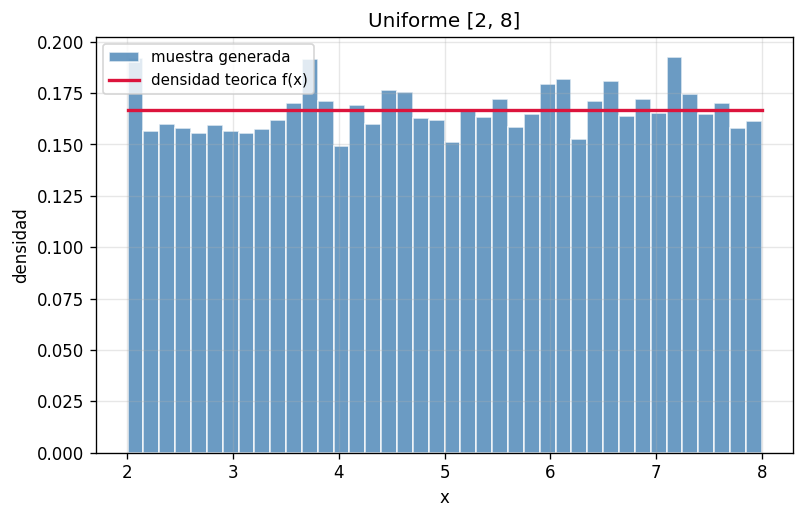
\includegraphics[width=\textwidth]{output/uniforme.png}
  \caption{Uniforme [2, 8]}
\end{subfigure}
\begin{subfigure}{0.48\textwidth}
  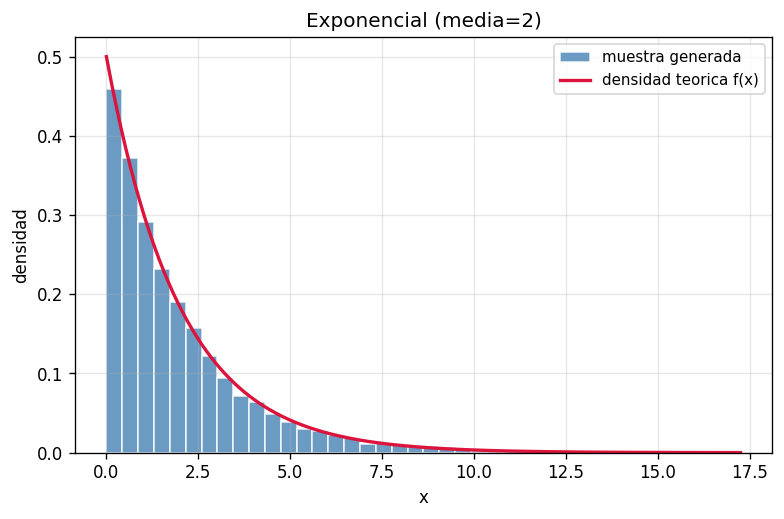
\includegraphics[width=\textwidth]{output/exponencial.png}
  \caption{Exponencial (media=2)}
\end{subfigure}
\\[0.5em]
\begin{subfigure}{0.48\textwidth}
  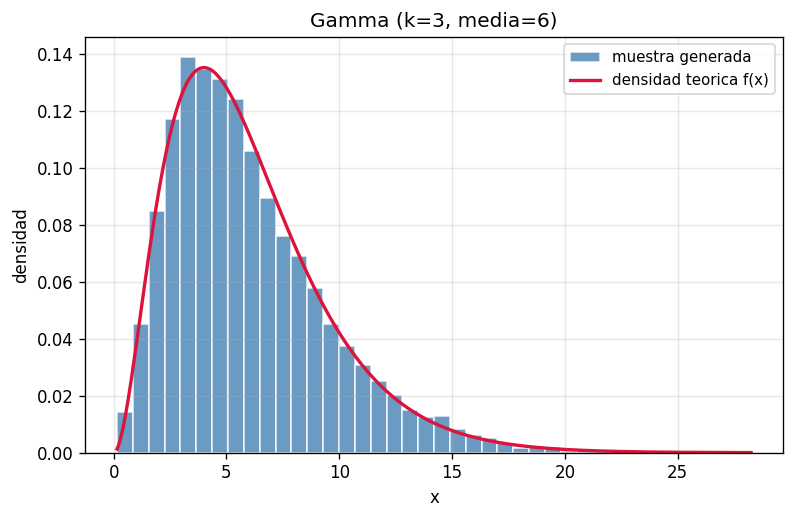
\includegraphics[width=\textwidth]{output/gamma.png}
  \caption{Gamma (k=3, media=6)}
\end{subfigure}
\begin{subfigure}{0.48\textwidth}
  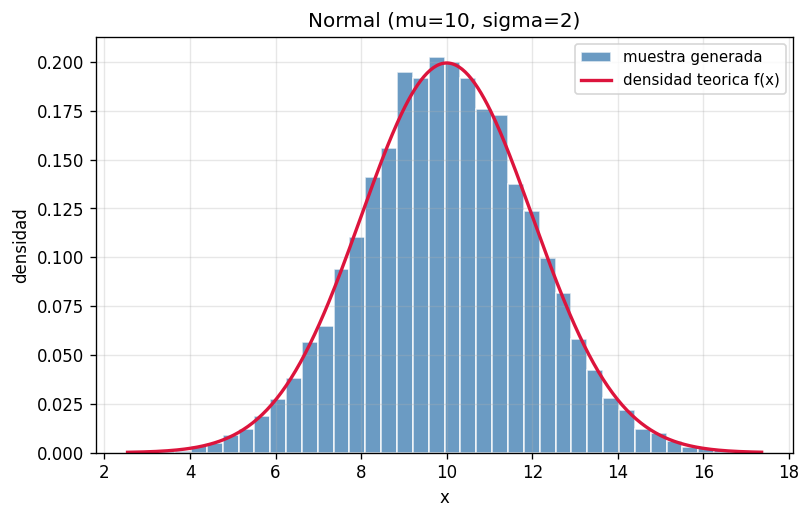
\includegraphics[width=\textwidth]{output/normal.png}
  \caption{Normal (mu=10, sigma=2)}
\end{subfigure}
\caption{Distribuciones continuas: histograma de la muestra generada
(azul) superpuesto con la densidad te\'orica $f(x)$ (rojo).}
\label{fig:continuas}
\end{figure}

\subsection{Gr\'aficos: discretas}

\begin{figure}[H]
\centering
\begin{subfigure}{0.48\textwidth}
  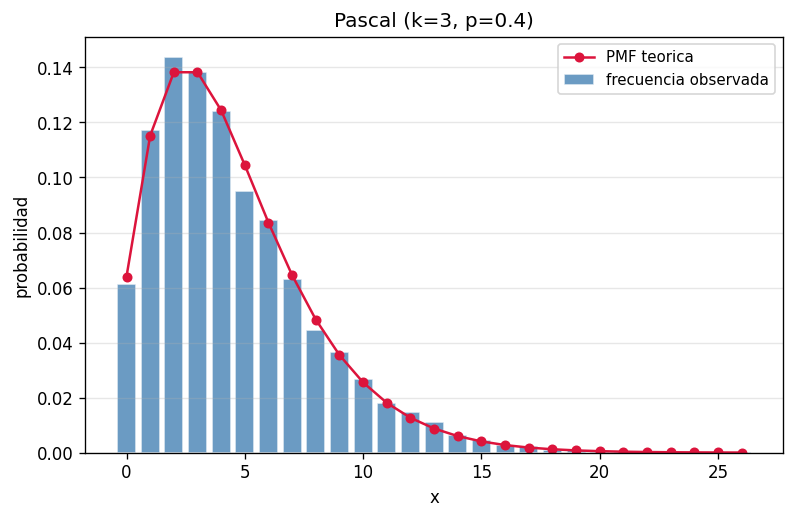
\includegraphics[width=\textwidth]{output/pascal.png}
  \caption{Pascal (k=3, p=0,4)}
\end{subfigure}
\begin{subfigure}{0.48\textwidth}
  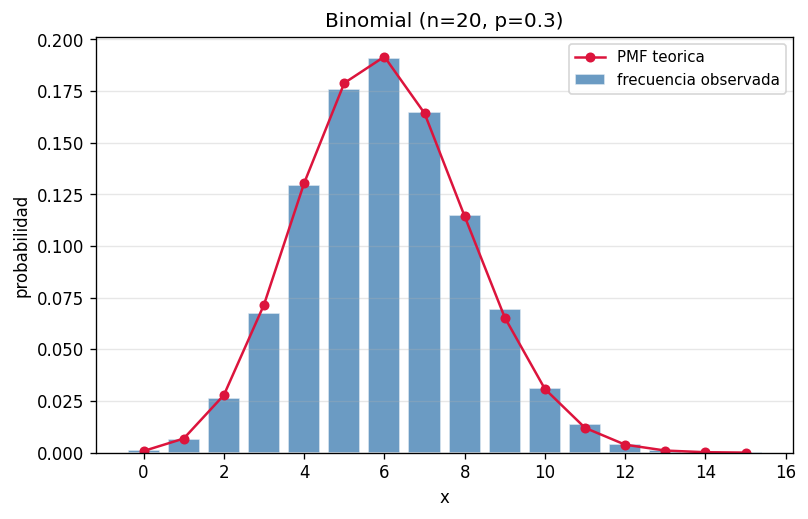
\includegraphics[width=\textwidth]{output/binomial.png}
  \caption{Binomial (n=20, p=0,3)}
\end{subfigure}
\\[0.5em]
\begin{subfigure}{0.48\textwidth}
  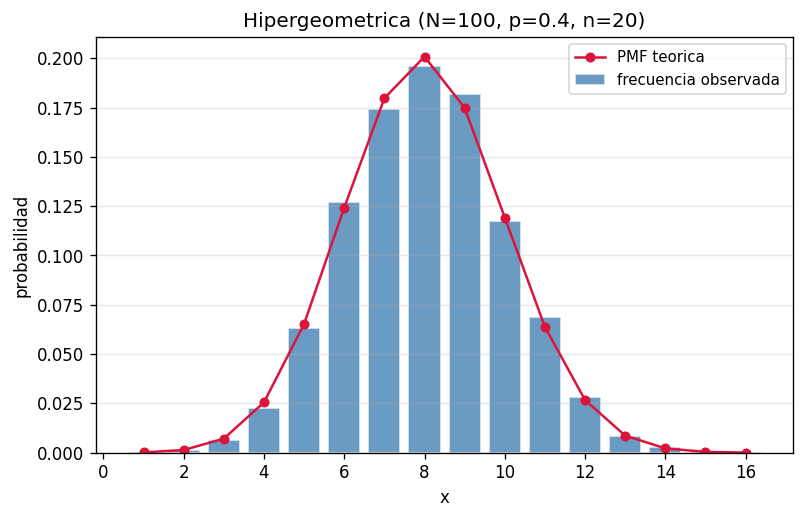
\includegraphics[width=\textwidth]{output/hipergeometrica.png}
  \caption{Hipergeom\'etrica (N=100, p=0,4, n=20)}
\end{subfigure}
\begin{subfigure}{0.48\textwidth}
  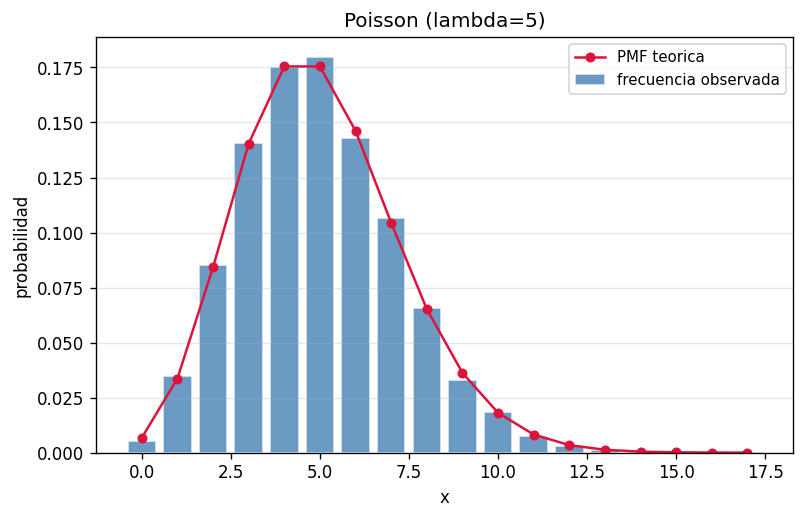
\includegraphics[width=\textwidth]{output/poisson.png}
  \caption{Poisson ($\lambda$=5)}
\end{subfigure}
\\[0.5em]
\begin{subfigure}{0.48\textwidth}
  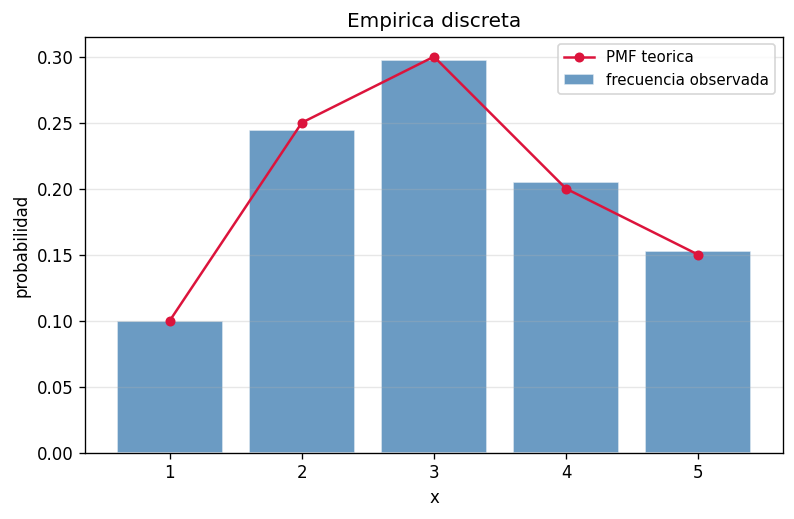
\includegraphics[width=\textwidth]{output/empirica.png}
  \caption{Emp\'irica discreta}
\end{subfigure}
\caption{Distribuciones discretas: frecuencia relativa observada (barras)
vs.\ funci\'on de probabilidad te\'orica PMF (puntos rojos).}
\label{fig:discretas}
\end{figure}

\section{Discusi\'on}

\textbf{Ajuste de las medias y varianzas.} La Tabla~\ref{tab:resultados}
muestra que, para las nueve distribuciones, las medias y varianzas
emp\'iricas coinciden con las te\'oricas con error menor al $5\%$. Las
peque\~nas desviaciones residuales (por ejemplo en la varianza de la gamma
o de la Pascal) son fluctuaciones de muestreo esperables para $n = 10000$ y
se reducen al aumentar el tama\~no de la muestra.

\textbf{El caso de la Pascal.} Durante el desarrollo se detect\'o que la
forma compacta de Naylor $x=\ln(\prod r_i)/\ln q$ con un \'unico redondeo
final sesgaba la media (daba $\approx 5{,}9$ en lugar de $4{,}5$). La causa
es que el redondeo debe aplicarse a cada geom\'etrica por separado, ya que
$\lfloor a\rfloor+\lfloor b\rfloor\neq\lfloor a+b\rfloor$. Corregido el
m\'etodo (suma de geom\'etricas redondeadas individualmente), la media
emp\'irica converge correctamente al valor te\'orico. Es un buen ejemplo de
que la implementaci\'on debe validarse siempre contra los momentos
te\'oricos.

\textbf{Pruebas de bondad de ajuste.} Las seis distribuciones exigidas
superan su prueba (Tabla~\ref{tab:tests}). Los $p$-valores, todos
holgadamente por encima de $0{,}05$, indican que no hay evidencia para
rechazar que las muestras provengan de la distribuci\'on te\'orica
correspondiente. La coincidencia de los $p$-valores de la uniforme y la
exponencial ($0{,}2967$) no es casual: ambas parten exactamente de la misma
secuencia de uniformes del GCL (mismo estado inicial) y la transformaci\'on
inversa es mon\'otona, por lo que el estad\'istico KS se preserva.

\textbf{Evidencia gr\'afica.} Las Figuras~\ref{fig:continuas} y
\ref{fig:discretas} confirman visualmente el ajuste: las densidades
te\'oricas trazan exactamente el contorno de los histogramas y las PMF
te\'oricas pasan por el extremo de cada barra de frecuencia observada.

\textbf{Sobre los m\'etodos.} El trabajo ilustra que no existe un \'unico
m\'etodo universal: la transformaci\'on inversa es \'optima cuando $F^{-1}$
es cerrada (uniforme, exponencial, emp\'irica); cuando no lo es, se recurre a
la convoluci\'on (gamma, Pascal), a transformaciones especiales (Box-Muller
para la normal) o a la reproducci\'on directa del proceso (binomial,
hipergeom\'etrica, Poisson). Todos comparten la misma materia prima: los
uniformes del GCL.

\section{Conclusiones}

\begin{enumerate}
  \item Se construyeron generadores para nueve distribuciones de
    probabilidad a partir de los uniformes del GCL del TP 2.1, aplicando los
    m\'etodos de Naylor (transformaci\'on inversa, convoluci\'on, rechazo y
    reproducci\'on directa del proceso).
  \item Las nueve distribuciones reproducen sus momentos te\'oricos (media y
    varianza) con error menor al $5\%$ para $n = 10000$.
  \item Las seis distribuciones que el enunciado exige testear superan su
    prueba de bondad de ajuste (Kolmogorov-Smirnov o chi-cuadrado) al nivel
    $\alpha = 0{,}05$.
  \item La validaci\'on contra los momentos te\'oricos result\'o esencial:
    permiti\'o detectar y corregir el sesgo en la generaci\'on de la Pascal
    derivado de un redondeo mal ubicado.
  \item El GCL validado en el TP 2.1 es una base s\'olida y suficiente para
    alimentar generadores de distribuciones arbitrarias, completando el
    estudio de los n\'umeros pseudoaleatorios necesario para los pr\'oximos
    experimentos de simulaci\'on.
\end{enumerate}

\begin{thebibliography}{9}

\bibitem{naylor}
Naylor, T. H. (1982). \emph{T\'ecnicas de simulaci\'on en computadoras}
(cap\'itulo 4: Generaci\'on de valores de las variables estoc\'asticas
empleadas en simulaci\'on). Limusa.

\bibitem{enunciado}
Torres, J. I. (2026). \emph{TP 2.2 - Generadores de n\'umeros
pseudoaleatorios de distintas distribuciones de probabilidad}. C\'atedra
Simulaci\'on, UTN FRRO.

\bibitem{boxmuller}
Box, G. E. P., \& Muller, M. E. (1958). A Note on the Generation of Random
Normal Deviates. \emph{Annals of Mathematical Statistics}, 29(2), 610-611.

\bibitem{ross}
Ross, S. M. (2019). \emph{Introducci\'on a la Probabilidad y la
Estad\'istica para Ingenieros y Cient\'ificos} (5\textsuperscript{a} ed.).
Academic Press.

\bibitem{walpole}
Walpole, R. E., Myers, R. H., Myers, S. L., \& Ye, K. (2012).
\emph{Probabilidad y Estad\'istica para Ingenieros y Ciencias}
(9\textsuperscript{a} ed.). Pearson.

\bibitem{matplotlib}
Hunter, J. D. (2007). Matplotlib: A 2D Graphics Environment.
\emph{Computing in Science \& Engineering}, 9(3), 90-95.

\bibitem{python}
Van Rossum, G., \& Drake, F. L. (2009). \emph{Python 3 Reference Manual}.
CreateSpace.

\end{thebibliography}

\end{document}
